% XCircuit output "hbusphys.tex" for LaTeX input from hbusphys.ps
\def\putbox#1#2#3#4{\makebox[0in][l]{\makebox[#1][l]{}\raisebox{\baselineskip}[0in][0in]{\raisebox{#2}[0in][0in]{\scalebox{#3}{#4}}}}}
\def\rightbox#1{\makebox[0in][r]{#1}}
\def\centbox#1{\makebox[0in]{#1}}
\def\topbox#1{\raisebox{-0.60\baselineskip}[0in][0in]{#1}}
\def\midbox#1{\raisebox{-0.20\baselineskip}[0in][0in]{#1}}
\begin{center}
   \scalebox{1}{
   \normalsize
   \parbox{4.63021in}{
   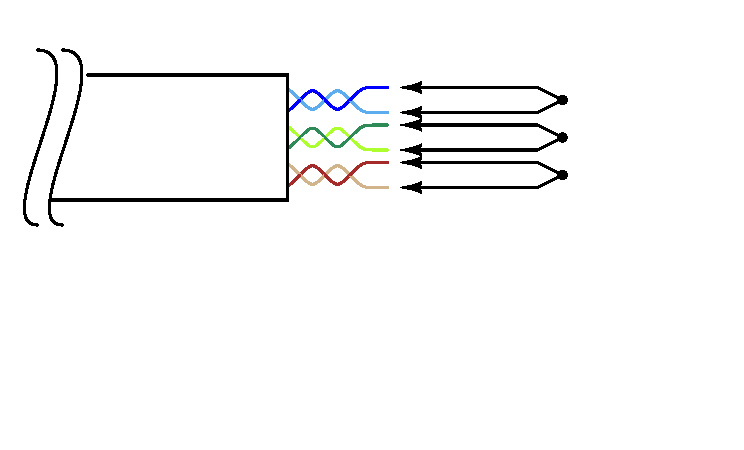
\includegraphics[scale=1,trim=0 1.5in 0 0]{hbusphys.ps}\\
   % translate x=1232 y=560 scale 0.38
   \putbox{4.06in}{2.72in}{1.20}{}%
   \putbox{1.64in}{0.06in}{1.20}{}%
   \putbox{4.56in}{0.97in}{1.20}{}%
   \putbox{3.72in}{0.72in}{1.20}{\midbox{RS485}}%
   \putbox{3.72in}{0.47in}{1.20}{\midbox{ALIMENTAÇÃO}}%
   \putbox{3.72in}{0.22in}{1.20}{\midbox{FREEBUS}}%
   } % close 'parbox'
   } % close 'scalebox'
   \vspace{-\baselineskip} % this is not necessary, but looks better
\end{center}
